\documentclass[titlepage]{article}
\usepackage{listings}
\lstMakeShortInline{|}
\usepackage{courier}
%\usepackage{hyperref}
\usepackage[colorlinks,linkcolor=blue,citecolor=blue,urlcolor=blue,breaklinks=true]{hyperref}
\lstset{basicstyle=\ttfamily\small , breaklines}
%\usepackage[margin=2cm]{geometry}
\usepackage[left=3cm,top=3cm,bottom=3cm, right=3cm,includehead,includefoot,landscape]{geometry}
\usepackage{color}
\usepackage{fancyhdr,lastpage}
\pagestyle{fancy}
\rhead{Metrum Research Group, LLC \\ }
\lhead{
\includegraphics[scale=2]{logo.png}}
\cfoot{Page \thepage\ of \pageref{LastPage}}
\fancyhfoffset{.25in}
\renewcommand{\headrulewidth}{0.25pt}
\renewcommand{\footrulewidth}{0pt} 
\setlength{\headheight}{23pt}
\renewcommand{\labelitemiii}{$\circ$}
\usepackage{longtable}
\usepackage{amsmath}
\usepackage[T1]{fontenc}
\usepackage[scaled]{helvet}
\renewcommand*\familydefault{\sfdefault}
\usepackage{courier}
\usepackage{graphicx}
\usepackage{tocbibind}
\usepackage[parfill]{parskip}    % Activate to begin paragraphs with an empty line rather than an indent
\usepackage{upgreek}
\usepackage{textpos}
\usepackage{relsize}
\usepackage{upquote}
% Use \begin{landscape} and end{landscape} to rotate text %%%
\usepackage{pdflscape}
\usepackage{textcomp}
\usepackage{float}
\floatplacement{figure}{H}
\floatplacement{table}{H}
\usepackage[printonlyused,nohyperlinks]{acronym}
\def\bflabel#1{{\large#1\ \ \ \ }\hfill}
\usepackage{fixltx2e}
\setlength{\belowcaptionskip}{10pt}





\usepackage{Sweave}

 
\begin{document}
\vspace*{2cm}
\begin{center}
{\Large Modeling}\\
~\\
\today\\
~\\
Tim Bergsma\\
\end{center}
\newpage

\section{Purpose}
This script runs NONMEM models and diagnostics for sample phase1 data.
\section{Model Development}
\subsection{Set up for NONMEM run.}
\begin{Schunk}
\begin{Sinput}
> #Be sure to set directory to the script directory that contains this file.
> library(metrumrg)
> command <- '/opt/NONMEM/nm73/nmqual/autolog.pl'
> cat.cov='SEX'
> cont.cov=c('HEIGHT','WEIGHT','AGE')
> par.list=c('CL','Q','KA','V','V2','V3')
> eta.list=paste('ETA',1:10,sep='')
\end{Sinput}
\end{Schunk}
\subsection{Run NONMEM.}
\begin{Schunk}
\begin{Sinput}
> NONR(
+      run=1001:1005,                       # 5 models, ctl pre-written
+      command=command,                    # this version will search for NONMEM
+      project='../nonmem',                 # must specify, unless ctl in getwd()
+      grid=TRUE,                          # set to FALSE for better error messaging (but slower)
+      nice=TRUE,                           # don't delete subversioned directories
+      checkrunno=FALSE,                    # TRUE auto-replaces conflicting run numbers
+      cont.cov=cont.cov,                   # see help for following
+      cat.cov=cat.cov,
+      par.list=par.list,
+      eta.list=eta.list,
+      grp='SEX',                           # separate diagnostic plots for each level of SEX
+      grpnames=c('female','male'),         # use these instead of 0, 1, when plotting by SEX
+      include.all=TRUE,                    # also show diagnostics with groups combined
+      plotfile='../nonmem/*/*.pdf',        # use the run dir and run name for the plot file 
+      streams='../nonmem/ctl'              # expect the control streams here, not locally
+ )
\end{Sinput}
\begin{Soutput}
Installing SIGCHLD signal handler...Done.
\end{Soutput}
\begin{Sinput}
> progress(1001:1005,project='../nonmem')
\end{Sinput}
\begin{Soutput}
       queued      compiled       running          done indeterminate 
            4             0             0             1             0 
\end{Soutput}
\begin{Sinput}
> follow(1001:1005,project='../nonmem')
\end{Sinput}
\begin{Soutput}
       queued      compiled       running          done indeterminate 
            4             0             0             1             0 
       queued      compiled       running          done indeterminate 
            0             5             0             0             0 
       queued      compiled       running          done indeterminate 
            0             3             1             1             0 
       queued      compiled       running          done indeterminate 
            0             0             2             3             0 
       queued      compiled       running          done indeterminate 
            0             0             0             5             0 
\end{Soutput}
\begin{Sinput}
> Sys.sleep(10)                             #wait briefly to ensure all processes complete
\end{Sinput}
\end{Schunk}
Covariance succeeded on model 1005.
We confirm that we can get similar results with different initial estimates.
\begin{Schunk}
\begin{Sinput}
> getwd()
\end{Sinput}
\begin{Soutput}
[1] "/data/metrumrg/inst/example/project/script"
\end{Soutput}
\begin{Sinput}
> ctl <- read.nmctl('../nonmem/1005/1005.ctl',parse=TRUE)
> names(ctl)
\end{Sinput}
\begin{Soutput}
 [1] "prob"       "input"      "data"       "subroutine" "pk"        
 [6] "error"      "theta"      "omega"      "sigma"      "estimation"
[11] "cov"        "table"      "table"     
\end{Soutput}
\begin{Sinput}
> ctl$theta[] <- lapply(ctl$theta,`comment<-`,value=NULL)
> writeLines(format(ctl$theta))
\end{Sinput}
\begin{Soutput}
; 
(0,10,50)
(0,10,100)
(0,0.2,5)
(0,10,50)
(0,100,1000)
(0,1,2)
(0,0.75,3)
\end{Soutput}
\begin{Sinput}
> set.seed(0)
> ctl$theta <- tweak(ctl$theta)
> writeLines(format(ctl$theta))
\end{Sinput}
\begin{Soutput}
; 
(0,11.6,50)
(0,9.58,100)
(0,0.235,5)
(0,11.7,50)
(0,105,1000)
(0,0.8,2)
(0,0.659,3)
\end{Soutput}
\begin{Sinput}
> ctl$prob
\end{Sinput}
\begin{Soutput}
[1] "1005 phase1 2 CMT like 1004 but diff. initial on V3"
\end{Soutput}
\begin{Sinput}
> ctl$prob <- '1006 like 1005 with tweaked initial estimates'
\end{Sinput}
\end{Schunk}
We request some variants of PRED and CWRES if running under NONMEM 7.3.
\begin{Schunk}
\begin{Sinput}
> ctl[[12]]
\end{Sinput}
\begin{Soutput}
[1] "NOPRINT FILE=./1005.tab ONEHEADER ID AMT TIME EVID PRED IPRE CWRES"
\end{Soutput}
\begin{Sinput}
> preds <- c('NPRED','CPRED','CPREDI','EPRED')
> res <- c('RES','NRES','NWRES','CRES','RESI','WRESI','CRESI','CWRESI','CIWRES','CIWRESI','ERES','EWRES','ECWRES')
> ctl[[12]] <- c(ctl[[12]],preds, res)
\end{Sinput}
\end{Schunk}
\begin{Schunk}
\begin{Sinput}
> write.nmctl(ctl,file='../nonmem/ctl/1006.ctl')
> NONR(
+      run=1006,
+      command=command,
+      project='../nonmem',
+      grid=TRUE,
+      nice=TRUE,
+      mode='para',                         # For illustrative purposes, we parallelize this run.
+      pe='orte 16',                        # orte is the parallelization environment; we use 16 cores.
+      checkrunno=TRUE,                     # default
+      diag=TRUE,                           # default
+      streams='../nonmem/ctl',             # software will look for 1006.pmn or template.pmn
+      plotfile='../nonmem/*/*.pdf',
+      epilog='../../misc/epilog.R',
+      eta.list='ETA1'
+ )
> Sys.sleep(5)
> qstat()
> follow(1006,project='../nonmem')
\end{Sinput}
\begin{Soutput}
       queued      compiled       running          done indeterminate 
            1             0             0             0             0 
       queued      compiled       running          done indeterminate 
            0             1             0             0             0 
       queued      compiled       running          done indeterminate 
            0             0             1             0             0 
       queued      compiled       running          done indeterminate 
            0             0             1             0             0 
       queued      compiled       running          done indeterminate 
            0             0             0             1             0 
\end{Soutput}
\begin{Sinput}
> Sys.sleep(20)
\end{Sinput}
\end{Schunk}
We can make a quick run log using some simple tools. Table \ref{runlog}.
\begin{Schunk}
\begin{Sinput}
> # intentionally including a bogus run, to test effect
> # don't want the 'wide' file, just the 'long' R object
> log <- rlog(1001:1007,'../nonmem',file=NULL) 
> head(log)
\end{Sinput}
\begin{Soutput}
  tool  run parameter   moment            value
1  nm7 1001       ofv  minimum 2526.39867049215
2  nm7 1001    THETA1 estimate          11.7167
3  nm7 1001    THETA1     prse             8.67
4  nm7 1001    THETA1       se           1.0163
5  nm7 1001    THETA2 estimate          14.5657
6  nm7 1001    THETA2     prse             8.67
\end{Soutput}
\begin{Sinput}
> tail(log)
\end{Sinput}
\begin{Soutput}
    tool  run parameter   moment                                         value
299  nm7 1006  SIGMA2.2       se                                     0.0675535
300  nm7 1006       cov   status                                             0
301  nm7 1006      prob     text 1006 like 1005 with tweaked initial estimates
302  nm7 1006       min   status                                             0
303  nm7 1006      data filename                 ../../data/derived/phase1.csv
304  nm7 1007       min   status                                            -1
\end{Soutput}
\begin{Sinput}
> sapply(log,class)
\end{Sinput}
\begin{Soutput}
       tool         run   parameter      moment       value 
"character"   "integer" "character" "character" "character" 
\end{Soutput}
\begin{Sinput}
> log$tool <- NULL
> log <- log[log$run!=1007,]
> unique(log$parameter)
\end{Sinput}
\begin{Soutput}
 [1] "ofv"      "THETA1"   "THETA2"   "THETA3"   "OMEGA1.1" "OMEGA2.1"
 [7] "OMEGA2.2" "OMEGA3.1" "OMEGA3.2" "OMEGA3.3" "SIGMA1.1" "SIGMA2.1"
[13] "SIGMA2.2" "cov"      "prob"     "min"      "data"     "THETA4"  
[19] "THETA5"   "OMEGA4.1" "OMEGA4.2" "OMEGA4.3" "OMEGA4.4" "OMEGA5.1"
[25] "OMEGA5.2" "OMEGA5.3" "OMEGA5.4" "OMEGA5.5" "THETA6"   "THETA7"  
\end{Soutput}
\begin{Sinput}
> log <- log[log$parameter %in% c('ofv','prob','cov','min'),]
> log
\end{Sinput}
\begin{Soutput}
     run parameter  moment
1   1001       ofv minimum
38  1001       cov  status
39  1001      prob    text
40  1001       min  status
42  1002       ofv minimum
112 1002       cov  status
113 1002      prob    text
114 1002       min  status
116 1003       ofv minimum
153 1003       cov  status
154 1003      prob    text
155 1003       min  status
157 1004       ofv minimum
194 1004       cov  status
195 1004      prob    text
196 1004       min  status
198 1005       ofv minimum
247 1005       cov  status
248 1005      prob    text
249 1005       min  status
251 1006       ofv minimum
300 1006       cov  status
301 1006      prob    text
302 1006       min  status
                                                          value
1                                              2526.39867049215
38                                                            0
39                                             1001 phase1 1CMT
40                                                            0
42                                             2525.96554218893
112                                                           1
113                                           1002 phase1 2 CMT
114                                                         134
116                                            2570.47417267741
153                                                           1
154 1003 phase1 2 CMT like 1002 but no eta on Q/v3 and no + err
155                                                         136
157                                            2570.45022474012
194                                                           1
195               1004 phase1 2 CMT like 1003 but better bounds
196                                                           0
198                                            2405.91626140177
247                                                           0
248         1005 phase1 2 CMT like 1004 but diff. initial on V3
249                                                           0
251                                            2405.91625717115
300                                                           0
301               1006 like 1005 with tweaked initial estimates
302                                                           0
\end{Soutput}
\begin{Sinput}
> with(log, constant(moment,within=parameter))#i.e., moment is non-informative here.
\end{Sinput}
\begin{Soutput}
[1] TRUE
\end{Soutput}
\begin{Sinput}
> log <- data.frame(cast(log,run~parameter))
> log <- shuffle(log,'prob','run')
> log$ofv <- signif(digits=6,as.numeric(as.character(log$ofv)))
\end{Sinput}
\end{Schunk}
\begin{table}[!htpb]
 \caption[Run Log]{Run Log \label{runlog}}
 \begin{center}
  \begin{tabular}{rlllr}
    \hline \hline
   run & prob & cov & min & ofv \\ \hline
   \verb#1001# & 1001 phase1 1CMT                                            & 0 & 0   & \verb#2526.40# \\
   \verb#1002# & 1002 phase1 2 CMT                                           & 1 & 134 & \verb#2525.97# \\
   \verb#1003# & 1003 phase1 2 CMT like 1002 but no eta on Q/v3 and no + err & 1 & 136 & \verb#2570.47# \\
   \verb#1004# & 1004 phase1 2 CMT like 1003 but better bounds               & 1 & 0   & \verb#2570.45# \\
   \verb#1005# & 1005 phase1 2 CMT like 1004 but diff. initial on V3         & 0 & 0   & \verb#2405.92# \\
   \verb#1006# & 1006 like 1005 with tweaked initial estimates               & 0 & 0   & \verb#2405.92# \\ \hline
  \end{tabular}
 \end{center}
\end{table}\section{Predictive Check}
\subsection{Create a simulation control stream.}
Convert control stream to R object.
\begin{Schunk}
\begin{Sinput}
> ctl <- read.nmctl('../nonmem/ctl/1005.ctl')
\end{Sinput}
\end{Schunk}
Strip comments and view.
\begin{Schunk}
\begin{Sinput}
> ctl[] <- lapply(ctl,function(rec)sub(' *;.*','',rec))          # read control stream into a list
> ctl                                                            # print it like text
\end{Sinput}
\begin{Soutput}
 [1] "$PROB 1005 phase1 2 CMT like 1004 but diff. initial on V3"                       
 [2] "$INPUT C ID TIME SEQ=DROP EVID AMT DV SUBJ HOUR HEIGHT WT SEX AGE DOSE FED"      
 [3] "$DATA ../../data/derived/phase1.csv IGNORE=C"                                    
 [4] "$SUBROUTINE ADVAN4 TRANS4"                                                       
 [5] "$PK"                                                                             
 [6] " CL=THETA(1)*EXP(ETA(1)) * THETA(6)**SEX * (WT/70)**THETA(7)"                    
 [7] " V2 =THETA(2)*EXP(ETA(2))"                                                       
 [8] " KA=THETA(3)*EXP(ETA(3))"                                                        
 [9] " Q  =THETA(4)"                                                                   
[10] " V3=THETA(5)"                                                                    
[11] " S2=V2"                                                                          
[12] " "                                                                               
[13] "$ERROR"                                                                          
[14] " Y=F*(1+ERR(1)) + ERR(2)"                                                        
[15] " IPRE=F"                                                                         
[16] ""                                                                                
[17] "$THETA"                                                                          
[18] "(0,10,50)"                                                                       
[19] "(0,10,100)"                                                                      
[20] "(0,0.2, 5)"                                                                      
[21] "(0,10,50)"                                                                       
[22] "(0,100,1000)"                                                                    
[23] "(0,1,2)"                                                                         
[24] "(0,0.75,3)"                                                                      
[25] ""                                                                                
[26] "$OMEGA BLOCK(3)"                                                                 
[27] ".1"                                                                              
[28] ".01 .1"                                                                          
[29] ".01 .01 .1"                                                                      
[30] ""                                                                                
[31] ""                                                                                
[32] ""                                                                                
[33] ""                                                                                
[34] ""                                                                                
[35] ""                                                                                
[36] ""                                                                                
[37] ""                                                                                
[38] "$SIGMA 0.1 0.1"                                                                  
[39] ""                                                                                
[40] ""                                                                                
[41] ""                                                                                
[42] ""                                                                                
[43] "$ESTIMATION MAXEVAL=9999 PRINT=5 NOABORT METHOD=1 INTER MSFO=./1005.msf"         
[44] "$COV PRINT=E"                                                                    
[45] "$TABLE NOPRINT FILE=./1005.tab ONEHEADER ID AMT TIME EVID PRED IPRE CWRES"       
[46] "$TABLE NOPRINT FILE=./1005par.tab ONEHEADER ID TIME CL Q V2 V3 KA ETA1 ETA2 ETA3"
[47] ""                                                                                
[48] ""                                                                                
[49] ""                                                                                
[50] ""                                                                                
[51] ""                                                                                
[52] ""                                                                                
[53] ""                                                                                
[54] ""                                                                                
[55] ""                                                                                
[56] ""                                                                                
[57] ""                                                                                
[58] ""                                                                                
[59] ""                                                                                
[60] ""                                                                                
[61] ""                                                                                
[62] ""                                                                                
[63] ""                                                                                
\end{Soutput}
\end{Schunk}
Fix records of interest.
\begin{Schunk}
\begin{Sinput}
> ctl$prob                                                       # problem statement
\end{Sinput}
\begin{Soutput}
[1] "1005 phase1 2 CMT like 1004 but diff. initial on V3"
\end{Soutput}
\begin{Sinput}
> ctl$prob <- sub('1005','1105',ctl$prob)                        # substitute new run number
> names(ctl)
\end{Sinput}
\begin{Soutput}
 [1] "prob"       "input"      "data"       "subroutine" "pk"        
 [6] "error"      "theta"      "omega"      "sigma"      "estimation"
[11] "cov"        "table"      "table"     
\end{Soutput}
\begin{Sinput}
> names(ctl)[names(ctl)=='theta'] <- 'msfi'                      # replace theta with final msfi
> ctl$msfi <- '=../1005/1005.msf'
> ctl$omega <- NULL                                              # drop omega, sigma
> ctl$sigma <- NULL
> names(ctl)[names(ctl)=='estimation'] <- 'simulation'           # simulate instead of estimate
> ctl$simulation <- 'ONLYSIM (1968) SUBPROBLEMS=500'             
> ctl$cov <- NULL                                                # drop covariance step
> ctl$table <- NULL                                              # replace multiple tables with one
> ctl$table <- NULL
> ctl$table <- 'DV NOHEADER NOPRINT FILE=./1105.tab FORWARD NOAPPEND' # only really need DV, save file space
> write.nmctl(ctl,'../nonmem/ctl/1105.ctl')
\end{Sinput}
\end{Schunk}
\subsection{Run the simulation.}
This run makes the predictions (simulations).
\begin{Schunk}
\begin{Sinput}
> NONR(
+      run=1105,
+      command=command,
+      project='../nonmem',
+      grid=TRUE,
+      nice=TRUE,
+      diag=FALSE,
+      streams='../nonmem/ctl'
+ )
> follow(1105,project='../nonmem')
\end{Sinput}
\begin{Soutput}
       queued      compiled       running          done indeterminate 
            0             0             0             0             1 
       queued      compiled       running          done indeterminate 
            0             1             0             0             0 
       queued      compiled       running          done indeterminate 
            0             1             0             0             0 
       queued      compiled       running          done indeterminate 
            0             0             1             0             0 
       queued      compiled       running          done indeterminate 
            0             0             1             0             0 
       queued      compiled       running          done indeterminate 
            0             0             1             0             0 
       queued      compiled       running          done indeterminate 
            0             0             0             1             0 
\end{Soutput}
\begin{Sinput}
> Sys.sleep(80) # let all processes complete
\end{Sinput}
\end{Schunk}
\subsection{Combine the original data and the simulation data.}
Now we fetch the results and integrate them with the other data.
\begin{Schunk}
\begin{Sinput}
> x <- superset(
+   run=1105,
+   project='../nonmem',
+   read.output=list(read.table,header=FALSE)
+ )
> x <- x[,c('SUBJ','TIME','DV','V1','1105')]
> read.nmctl('../nonmem/1105/1105.ctl')$simulation
\end{Sinput}
\begin{Soutput}
[1] "ONLYSIM (1968) SUBPROBLEMS=500"
\end{Soutput}
\begin{Sinput}
> x$SIM <- rep(1:500,each=nrow(x)/500)
> colname(x) <- c(V1='PRED')
> x <- x[x$`1105`==1,]
> x$`1105` <- NULL
> head(x)
\end{Sinput}
\begin{Soutput}
  SUBJ TIME    DV    PRED SIM
2    1 0.00     . 0.00000   1
3    1 0.25 0.363 0.72576   1
4    1 0.50 0.914 1.38380   1
5    1 1.00  1.12 2.06800   1
6    1 2.00  2.28 3.48710   1
7    1 3.00  1.63 5.44790   1
\end{Soutput}
\begin{Sinput}
> nrow(x)
\end{Sinput}
\begin{Soutput}
[1] 275000
\end{Soutput}
\begin{Sinput}
> str(x)
\end{Sinput}
\begin{Soutput}
'data.frame':	275000 obs. of  5 variables:
 $ SUBJ: int  1 1 1 1 1 1 1 1 1 1 ...
 $ TIME: num  0 0.25 0.5 1 2 3 4 6 8 12 ...
 $ DV  : chr  "." "0.363" "0.914" "1.12" ...
 $ PRED: num  0 0.726 1.384 2.068 3.487 ...
 $ SIM : int  1 1 1 1 1 1 1 1 1 1 ...
\end{Soutput}
\begin{Sinput}
> x <- x[x$DV != '.',]
> x$DV <- as.numeric(x$DV)
\end{Sinput}
\end{Schunk}
\subsection{Plot predictive checks.}
\subsubsection{Aggregate data within subject.}
Since subjects may contribute differing numbers of observations, it may
be useful to look at predictions from a subject-centric perspective.
Therefore, we wish to calculate summary statistics for each subject, 
(observed and predicted) and then make obspred comparisons therewith.
\begin{Schunk}
\begin{Sinput}
> head(x)
\end{Sinput}
\begin{Soutput}
  SUBJ TIME    DV    PRED SIM
3    1 0.25 0.363 0.72576   1
4    1 0.50 0.914 1.38380   1
5    1 1.00 1.120 2.06800   1
6    1 2.00 2.280 3.48710   1
7    1 3.00 1.630 5.44790   1
8    1 4.00 2.040 2.99230   1
\end{Soutput}
\begin{Sinput}
> subject <- melt(x,measure.var=c('DV','PRED'))
> head(subject)
\end{Sinput}
\begin{Soutput}
  SUBJ TIME SIM variable value
1    1 0.25   1       DV 0.363
2    1 0.50   1       DV 0.914
3    1 1.00   1       DV 1.120
4    1 2.00   1       DV 2.280
5    1 3.00   1       DV 1.630
6    1 4.00   1       DV 2.040
\end{Soutput}
\end{Schunk}
We are going to aggregate each subject's DV and PRED values using cast().
cast() likes an aggregation function that returns a list.
We write one that grabs min med max for each subject, sim, and variable.
\begin{Schunk}
\begin{Sinput}
> metrics <- function(x)list(min=min(x), med=median(x), max=max(x))
\end{Sinput}
\end{Schunk}
Now we cast, ignoring time.
\begin{Schunk}
\begin{Sinput}
> subject <- data.frame(cast(subject, SUBJ + SIM + variable ~ .,fun=metrics))
> head(subject)
\end{Sinput}
\begin{Soutput}
  SUBJ SIM variable       min    med     max
1    1   1       DV  0.363000 1.6100  3.0900
2    1   1     PRED  0.725760 3.4805  5.4479
3    1   2       DV  0.363000 1.6100  3.0900
4    1   2     PRED -0.085183 2.2938  4.6454
5    1   3       DV  0.363000 1.6100  3.0900
6    1   3     PRED -0.022076 4.8891 12.3770
\end{Soutput}
\end{Schunk}
Note that regardless of SIM, DV (observed) is constant.

Now we melt the metrics.
\begin{Schunk}
\begin{Sinput}
> metr <- melt(subject,measure.var=c('min','med','max'),variable_name='metric')
> head(metr)
\end{Sinput}
\begin{Soutput}
  SUBJ SIM variable metric     value
1    1   1       DV    min  0.363000
2    1   1     PRED    min  0.725760
3    1   2       DV    min  0.363000
4    1   2     PRED    min -0.085183
5    1   3       DV    min  0.363000
6    1   3     PRED    min -0.022076
\end{Soutput}
\begin{Sinput}
> metr$value <- reapply(
+ 	metr$value,
+ 	INDEX=metr[,c('SIM','variable','metric')],
+ 	FUN=sort,
+ 	na.last=FALSE
+ )
> metr <- data.frame(cast(metr))
> head(metr)
\end{Sinput}
\begin{Soutput}
  SUBJ SIM metric    DV     PRED
1    1   1    min 0.139 -0.61532
2    1   1    med 1.025  1.25850
3    1   1    max 2.530  2.17590
4    1   2    min 0.139 -0.35190
5    1   2    med 1.025  1.20924
6    1   2    max 2.530  2.42400
\end{Soutput}
\begin{Sinput}
> nrow(metr)
\end{Sinput}
\begin{Soutput}
[1] 60000
\end{Soutput}
\begin{Sinput}
> metr <- metr[!is.na(metr$DV),]#maybe no NA
> nrow(metr)
\end{Sinput}
\begin{Soutput}
[1] 60000
\end{Soutput}
\end{Schunk}
We plot using lattice.
\begin{Schunk}
\begin{Sinput}
> print(
+ 	xyplot(
+ 		PRED~DV|metric,
+ 		metr,
+ 		groups=SIM,
+ 		scales=list(relation='free'),
+ 		type='l',
+ 		panel=function(...){
+ 			panel.superpose(...)
+ 			panel.abline(0,1,col='white',lwd=2)
+ 		}
+ 	)
+ )
\end{Sinput}
\end{Schunk}
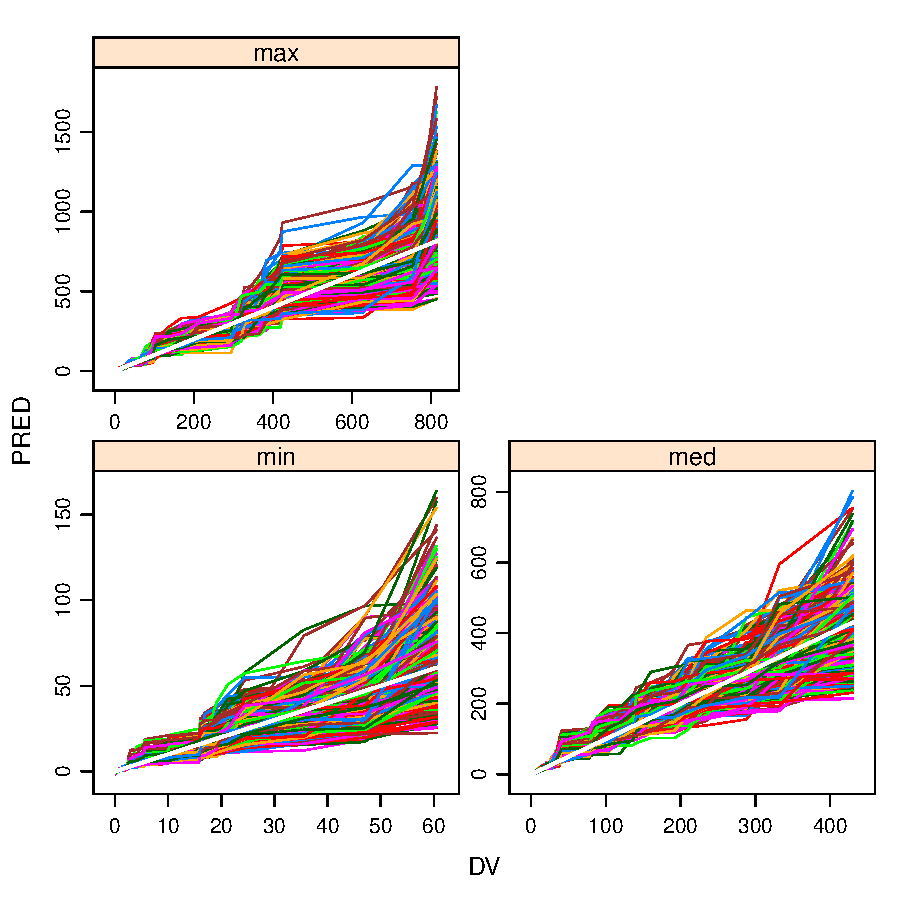
\includegraphics{model-qq}

For detail, we show one endpoint, tossing the outer 5 percent of values, and 
indicating quartiles. Technically, though, one may want to calculate quartiles
befor trimming the data.
\begin{Schunk}
\begin{Sinput}
> med <- metr[metr$metric=='med',]
> med$metric <- NULL
> head(med)
\end{Sinput}
\begin{Soutput}
   SUBJ SIM    DV    PRED
2     1   1 1.025 1.25850
5     1   2 1.025 1.20924
8     1   3 1.025 1.57950
11    1   4 1.025 0.88477
14    1   5 1.025 1.65875
17    1   6 1.025 0.95005
\end{Soutput}
\begin{Sinput}
> trim <- inner(med, id.var=c('SIM'),measure.var=c('PRED','DV'))
> head(trim)
\end{Sinput}
\begin{Soutput}
  SIM DV PRED
1   1 NA   NA
2   2 NA   NA
3   3 NA   NA
4   4 NA   NA
5   5 NA   NA
6   6 NA   NA
\end{Soutput}
\begin{Sinput}
> nrow(trim)
\end{Sinput}
\begin{Soutput}
[1] 20000
\end{Soutput}
\begin{Sinput}
> trim <- trim[!is.na(trim$DV),]
> nrow(trim)
\end{Sinput}
\begin{Soutput}
[1] 19000
\end{Soutput}
\begin{Sinput}
> head(trim)
\end{Sinput}
\begin{Soutput}
    SIM   DV     PRED
501   1 1.13 2.058700
502   2 1.13 2.005300
503   3 1.13 1.654800
504   4 1.13 1.069000
505   5 1.13 2.059750
506   6 1.13 0.985885
\end{Soutput}
\begin{Sinput}
> print(
+ 	xyplot(
+ 		PRED~DV,
+ 		trim,
+ 		groups=SIM,
+ 		type='l',
+ 		panel=function(x,y,...){
+ 			panel.xyplot(x=x,y=y,...)
+ 			panel.abline(0,1,col='white',lwd=2)
+ 			panel.abline(
+ 				v=quantile(x,probs=c(0.25,0.5,0.75)),
+ 				col='grey',
+ 				lty=2
+ 			)
+ 		}
+ 	)
+ )
\end{Sinput}
\end{Schunk}
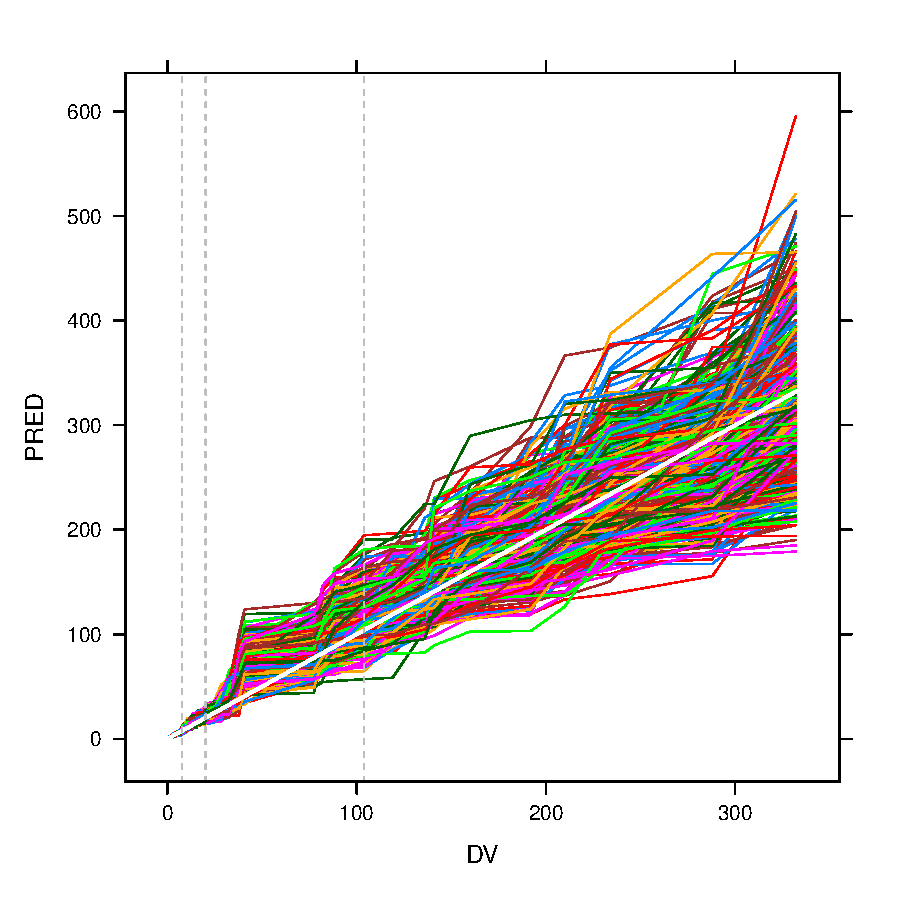
\includegraphics{model-qqdetail}

We also show densityplots of predictions at those quartiles.
\begin{Schunk}
\begin{Sinput}
> head(trim)
\end{Sinput}
\begin{Soutput}
    SIM   DV     PRED
501   1 1.13 2.058700
502   2 1.13 2.005300
503   3 1.13 1.654800
504   4 1.13 1.069000
505   5 1.13 2.059750
506   6 1.13 0.985885
\end{Soutput}
\begin{Sinput}
> quantile(trim$DV)
\end{Sinput}
\begin{Soutput}
    0%    25%    50%    75%   100% 
  1.13   7.69  20.25 104.00 332.00 
\end{Soutput}
\begin{Sinput}
> molt <- melt(trim, id.var='SIM')
> head(molt)
\end{Sinput}
\begin{Soutput}
  SIM variable value
1   1       DV  1.13
2   2       DV  1.13
3   3       DV  1.13
4   4       DV  1.13
5   5       DV  1.13
6   6       DV  1.13
\end{Soutput}
\begin{Sinput}
> quart <- data.frame(cast(molt,SIM+variable~.,fun=quantile,probs=c(0.25,0.5,0.75)))
> head(quart)
\end{Sinput}
\begin{Soutput}
  SIM variable      X25.     X50.      X75.
1   1       DV  7.950000 20.25000 100.10000
2   1     PRED 11.929000 22.16550 103.96000
3   2       DV  7.950000 20.25000 100.10000
4   2     PRED  7.234725 20.27300 105.19700
5   3       DV  7.950000 20.25000 100.10000
6   3     PRED  7.826900 14.50475  98.27925
\end{Soutput}
\begin{Sinput}
> molt <- melt(quart,id.var='variable',measure.var=c('X25.','X50.','X75.'),variable_name='quartile')
> head(molt)
\end{Sinput}
\begin{Soutput}
  variable quartile     value
1       DV     X25.  7.950000
2     PRED     X25. 11.929000
3       DV     X25.  7.950000
4     PRED     X25.  7.234725
5       DV     X25.  7.950000
6     PRED     X25.  7.826900
\end{Soutput}
\begin{Sinput}
> levels(molt$quartile)
\end{Sinput}
\begin{Soutput}
[1] "X25." "X50." "X75."
\end{Soutput}
\begin{Sinput}
> levels(molt$quartile) <- c('first quartile','second quartile','third quartile')
> head(molt)
\end{Sinput}
\begin{Soutput}
  variable       quartile     value
1       DV first quartile  7.950000
2     PRED first quartile 11.929000
3       DV first quartile  7.950000
4     PRED first quartile  7.234725
5       DV first quartile  7.950000
6     PRED first quartile  7.826900
\end{Soutput}
\begin{Sinput}
> levels(molt$variable)
\end{Sinput}
\begin{Soutput}
[1] "DV"   "PRED"
\end{Soutput}
\begin{Sinput}
> molt$variable <- factor(molt$variable,levels=c('PRED','DV'))
> print(
+ 	densityplot(
+ 		~value|quartile,
+ 		molt,
+ 		groups=variable,
+ 		layout=c(3,1),
+ 		scales=list(relation='free'),
+ 		aspect=1,
+ 		panel=panel.superpose,
+ 		panel.groups=function(x,...,group.number){
+ 			if(group.number==1)panel.densityplot(x,...)
+ 			if(group.number==2)panel.abline(v=unique(x),...)
+ 		},
+ 		auto.key=TRUE
+ 	)
+ )
\end{Sinput}
\end{Schunk}
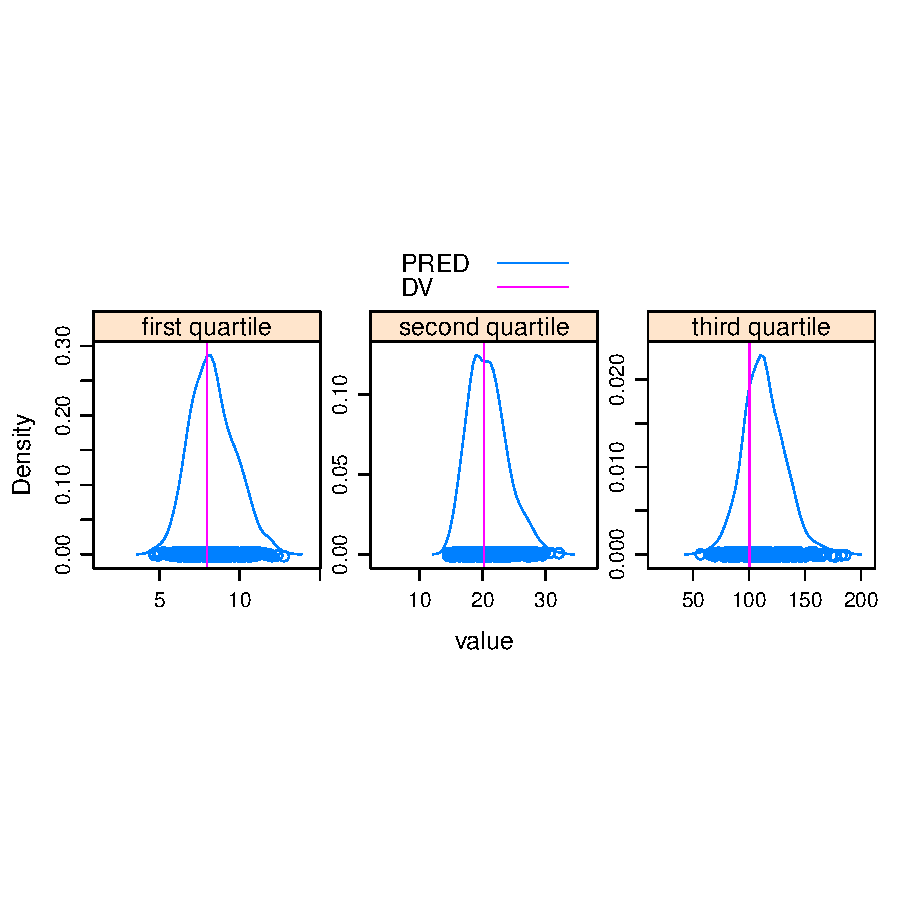
\includegraphics{model-qqdensity}
\section{Bootstrap Estimates of Parameter Uncertainty}
\subsection{Create directories.}
\begin{Schunk}
\begin{Sinput}
> getwd()
\end{Sinput}
\begin{Soutput}
[1] "/data/metrumrg/inst/example/project/script"
\end{Soutput}
\begin{Sinput}
> dir.create('../nonmem/1005boot')
> dir.create('../nonmem/1005bootdata')
> dir.create('../nonmem/1005bootctl')
\end{Sinput}
\end{Schunk}
\subsection{Create replicate control streams.}
\begin{Schunk}
\begin{Sinput}
> ctl <- clear(readLines('../nonmem/ctl/1005.ctl'),';.+',fixed=FALSE)
> #ctl <- read.nmctl('../nonmem/1005/1005.ctl')
> ctl <- as.nmctl(ctl)
> names(ctl)
\end{Sinput}
\begin{Soutput}
 [1] "prob"       "input"      "data"       "subroutine" "pk"        
 [6] "error"      "theta"      "omega"      "sigma"      "estimation"
[11] "cov"        "table"      "table"     
\end{Soutput}
\begin{Sinput}
> ctl$cov <- NULL
> ctl$table <- NULL
> ctl$table <- NULL
> ctl$prob
\end{Sinput}
\begin{Soutput}
[1] "1005 phase1 2 CMT like 1004 but diff. initial on V3"
\end{Soutput}
\begin{Sinput}
> ctl$data
\end{Sinput}
\begin{Soutput}
[1] "../../data/derived/phase1.csv IGNORE=C"
\end{Soutput}
\begin{Sinput}
> #makes nice padded run directories like 001 instead of 1 (better directory sorting) to be used below
> RUN <- padded(1:300) 
> invisible(
+   lapply(
+     RUN,
+     function(i,ctl){
+       ctl$prob <- sub('1005',i,ctl$prob)
+       ctl$data <- sub(
+         '../../data/derived/phase1.csv',
+         sub('\\*',i,'../../1005bootdata/*.csv'),
+         ctl$data
+       )
+       write.nmctl(ctl,file=glue('../nonmem/1005bootctl/',i,'.ctl'))
+     },
+     ctl=ctl
+   )
+ )
\end{Sinput}
\end{Schunk}
\subsection{Create replicate data sets by resampling original.}
\begin{Schunk}
\begin{Sinput}
>  bootset <- read.csv('../data/derived/phase1.csv')
>  r <- resample(
+  	bootset,
+  	names=RUN,
+  	key='ID',
+  	rekey=TRUE,
+  	out='../nonmem/1005bootdata',
+  	stratify='SEX'
+  )
\end{Sinput}
\end{Schunk}
\subsection{Run bootstrap models.}
\begin{Schunk}
\begin{Sinput}
> #intentionally trying a non-existent run ... 1 should be 001 per above. 
> #Parentheses force display of invisible NONR result.
> (NONR(
+      run=1,
+      wait=FALSE,
+      grid=TRUE,
+      project='../nonmem/1005boot',
+      streams='../nonmem/1005bootctl',
+      command=command
+ ))
\end{Sinput}
\begin{Soutput}
[[1]]
[1] "../nonmem/1005bootctl/1.ctl not found"
\end{Soutput}
\begin{Sinput}
> NONR(
+      run=RUN,
+      wait=FALSE,
+      grid=TRUE,
+      project='../nonmem/1005boot',
+      streams='../nonmem/1005bootctl',
+      command=command
+ )
> qstat()
> follow(RUN,project='../nonmem/1005boot')
\end{Sinput}
\begin{Soutput}
       queued      compiled       running          done indeterminate 
          164            56            10            70             0 
       queued      compiled       running          done indeterminate 
          147            48            25            80             0 
       queued      compiled       running          done indeterminate 
          140            14            58            88             0 
       queued      compiled       running          done indeterminate 
          114            31            29           126             0 
       queued      compiled       running          done indeterminate 
           83            37            34           145             1 
       queued      compiled       running          done indeterminate 
           61            39            25           174             1 
       queued      compiled       running          done indeterminate 
           36            27            40           197             0 
       queued      compiled       running          done indeterminate 
           16            30            36           218             0 
       queued      compiled       running          done indeterminate 
            0            16            42           242             0 
       queued      compiled       running          done indeterminate 
            0             0            17           283             0 
       queued      compiled       running          done indeterminate 
            0             0             0           300             0 
\end{Soutput}
\begin{Sinput}
> Sys.sleep(5)
> boot <- rlog(
+ 	run=RUN,
+ 	project='../nonmem/1005boot',
+ 	append=FALSE,
+ 	tool='nm7',
+   file=NULL
+ )
> write.csv(boot, '../nonmem/1005bootlog.csv')
> Sys.sleep(5)
\end{Sinput}
\end{Schunk}
\section{File Disposition}
Predictive checks and bootstraps make huge files that need not be retained.
\begin{Schunk}
\begin{Sinput}
> unlink('../nonmem/1105',recursive=TRUE)
> unlink('../nonmem/1005boot',recursive=TRUE)
> unlink('../nonmem/1005bootdata',recursive=TRUE)
> unlink('../nonmem/1005bootctl',recursive=TRUE)
\end{Sinput}
\end{Schunk}
\end{document}
